%--------------------------------------------------------
%--------------------------------------------------------
\subsection{Application to Planck 353 Ghz polarization maps}
%
\begin{figure}[!h] 
\centering
\subfigure[]{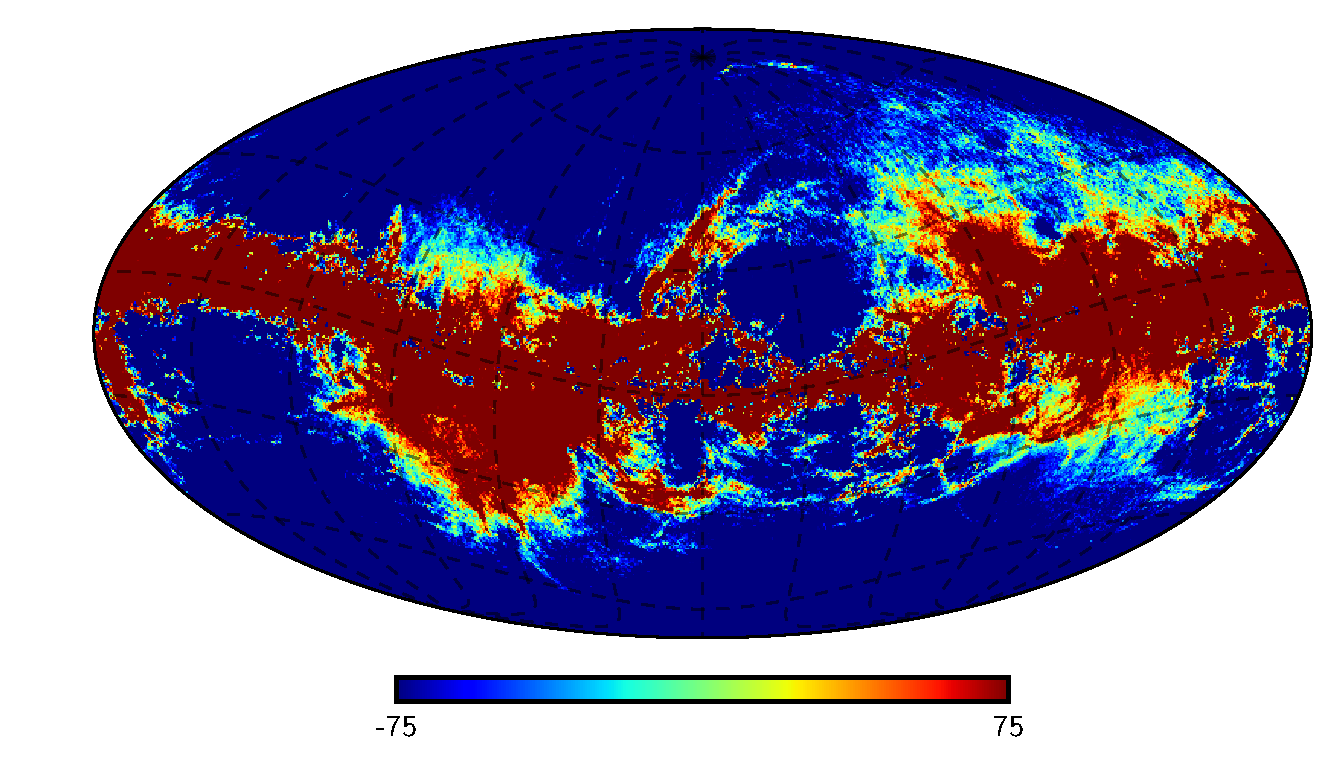
\includegraphics[width=0.49\columnwidth]{353ghz/353ghz-e-mode-healpix.pdf}}
\subfigure[]{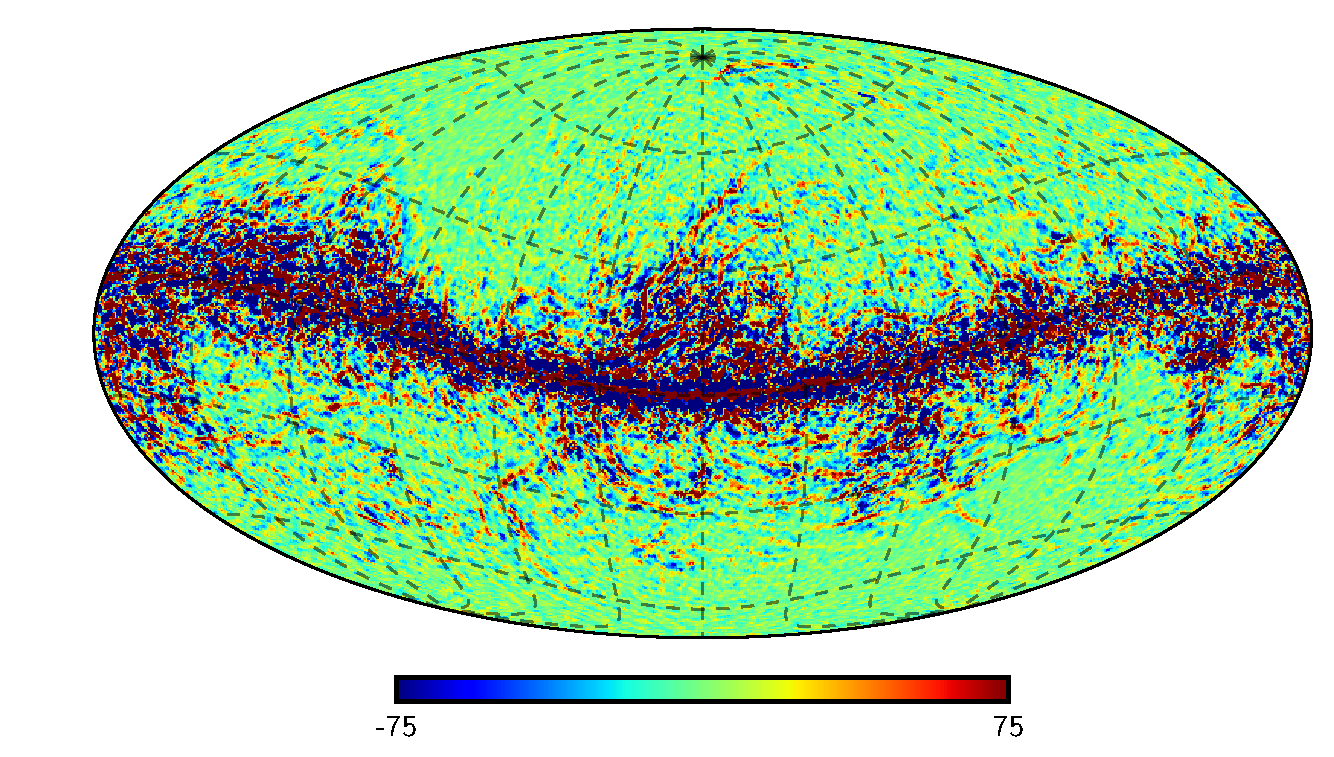
\includegraphics[width=0.49\columnwidth]{353ghz/353ghz-e-mode-real-space-disc8apo3.pdf}}
\subfigure[]{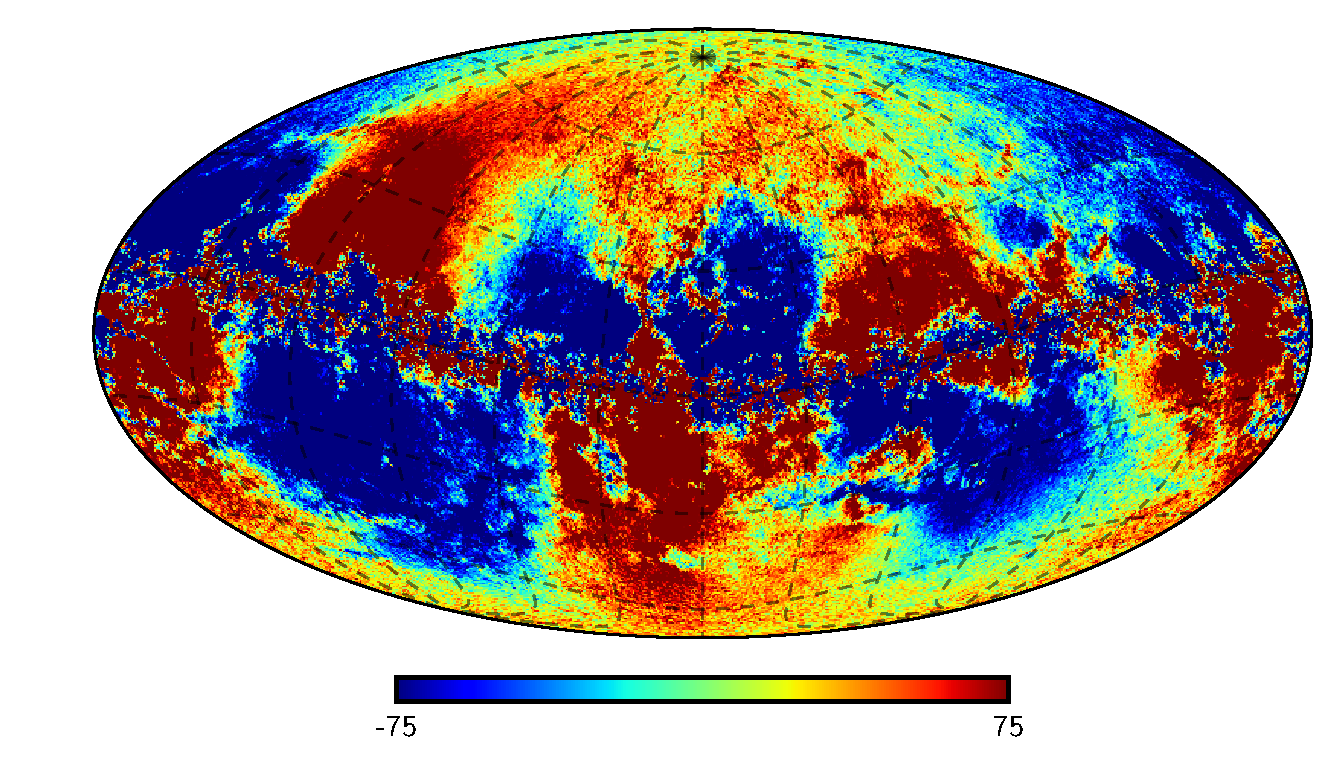
\includegraphics[width=0.49\columnwidth]{353ghz/353ghz-b-mode-healpix.pdf}}
\subfigure[]{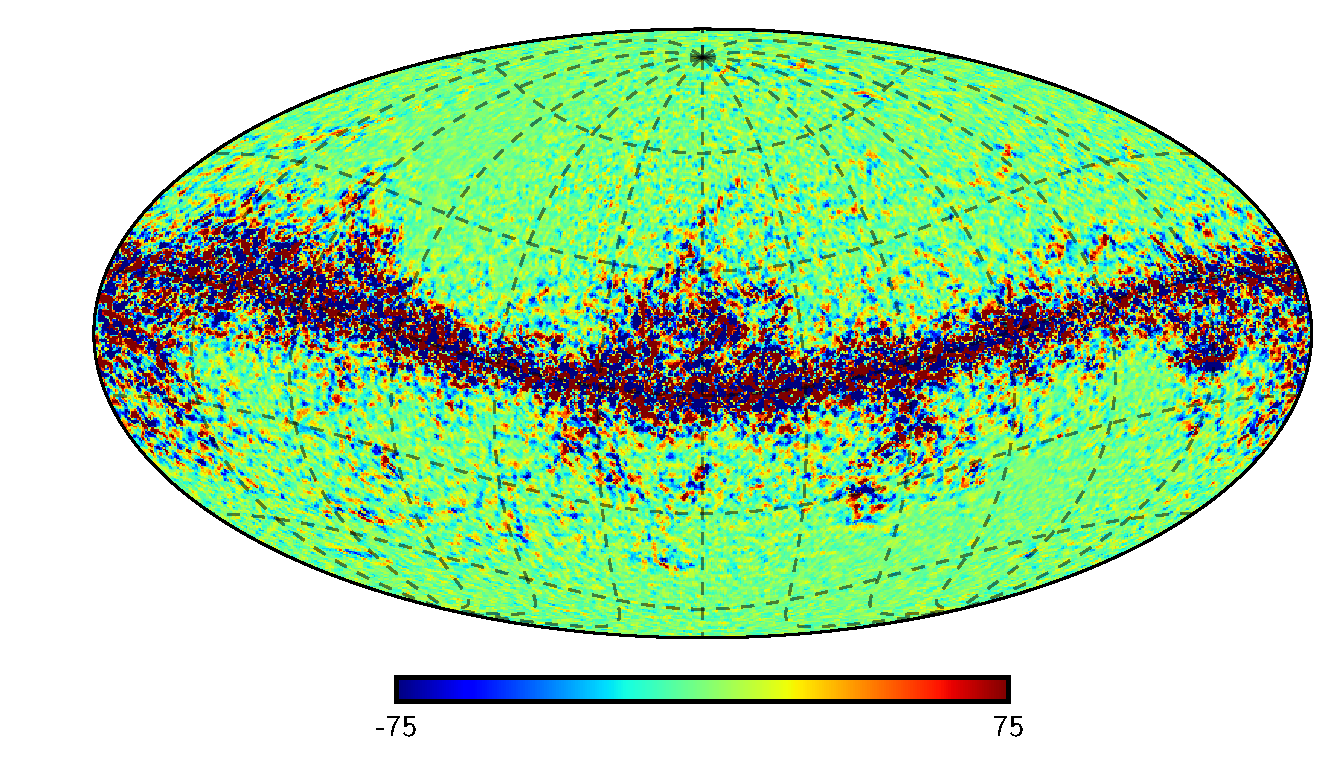
\includegraphics[width=0.49\columnwidth]{353ghz/353ghz-b-mode-real-space-disc8apo3.pdf}}
\caption{}
\label{fig:353ghz-eb-maps}
\end{figure}
%
%--------------------------------------------------------
%--------------------------------------------------------

%--------------------------------------------------------
%--------------------------------------------------------
\subsection{Scaling and future prospects}
%
\begin{figure}[!h] 
\centering
\subfigure[]{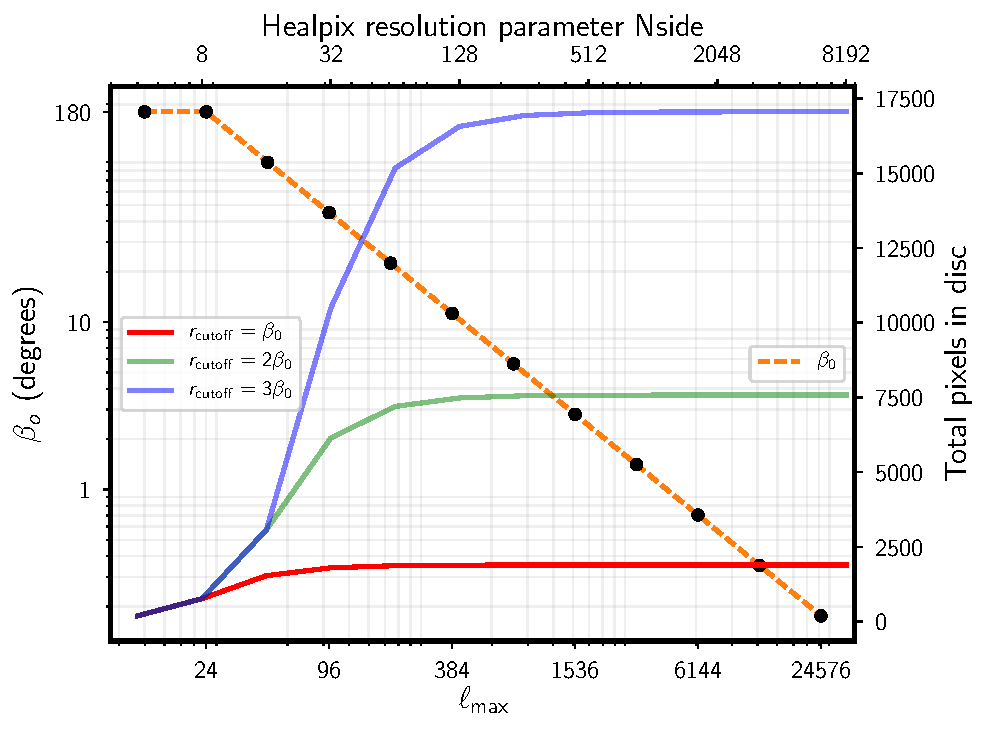
\includegraphics[width=0.8\columnwidth]{supplementary/number_of_disc_pixels.pdf}}
\caption{The red dashed curve depicts the how $\beta_o$ changes as a function of the Healpix resolution parameter Nside assuming that the maximum multipole accessible in the map is given by $\ell_{\rm max} = 3 * Nside$. The blue solid curve depicts the number of surrounding pixel that will need to be accessed to carry out the convolution on Stokes Q \& U maps to infer the value of the scalar fields E \& B at the central pixel.}
\label{fig:disc_rad_healpix_numpix}
\end{figure}
%
%--------------------------------------------------------
%--------------------------------------------------------
